\documentclass[11pt]{report}
\usepackage[a4paper]{geometry}
\usepackage{outline}
\usepackage{pmgraph}
\usepackage[normalem]{ulem}
\usepackage{graphicx}
\usepackage{booktabs}
\usepackage{amsmath}
\usepackage{amsthm}
\usepackage{eucal}
\usepackage{amssymb}
\usepackage{mathrsfs}
\begin{document}
\chapter{PageRank beyond the web - Gleich}
\begin{itemize}
\item Biology - GeneRank
\item PageRank used as a network centrality measure - help understand graph better by focusing on what PageRank reveals as important
\item Used to illuminate a region of a large graph around a target set of interest - localized measure, personalized PageRank
\item Reverse PageRank - follow inlinks instead of outlinks
\end{itemize}
\section{Chemistry}
\begin{itemize}
\item Valence of a molecule is the number of potential bonds it can make
\item PageRank to study molecules in chemistry - Mooney et al 2002
\item Use PageRank to assess the change in a network of molecules linked by hydrogen bonds among water molecules
\item Graph contains edges between water molecules if they have a potential hydrogen bond to a solute molecule
\item Goal to assess the hydrogen bond potential of a solvent
\item REFERENCE: \textbf{B. L. Mooney, L. R. Corrales, and A. E. Clark}, \textit{Molecularnetworks: An integrated graph
theoretic and data mining tool to explore solvent organization in molecular simulation.}
\end{itemize}
\section{Neuroscience}
\begin{itemize}
\item Evaluate the importance of brain regions given observed correlations of brain activity
\end{itemize}
\section{Roads and Urban spaces}
\begin{itemize}
\item Predict both traffic flow and human movement
\item Natural road - continuous path built from road segments joining adjacent segments together
\item PageRank with $\alpha=0.95$ , Jiang et al, PageRank best network measure in terms of predicting traffic on individual roads - 15000 nodes and 50000 edges
\item REFERENCE:\textbf{B. Jiang, S. Zhao, and J. Yin}, \textit{Self-organized natural roads for predicting traffic flow: a sensitivity
study}
\item Urban spaces - largest space of a city observable from a single vantage point - Jiang 2009, urban space best considered as a city neighbourhood or block
\item Urban space network connects adjacent spaces, or blocks, if physically adjacent
\item Urban spaces in London have up to 20000 nodes and 100000 links
\item Weighted PageRank best predicts human mobility in London - $\alpha=1$ accounts for up to 60\% of movement
\item Individuals cannot teleport
\item REFERENCE:\textbf{B. Jiang}, \textit{Ranking spaces for predicting human movement in an urban environment}
\end{itemize}
\section{Sports}
\begin{itemize}
\item Winner network
\item Idea underlying these rankings is that of a random fan that follows a team until another team beats them, at which point they pick up the new team, and periodically restarts with an arbitrary team
\end{itemize}
\section{ItemRank}
\begin{itemize}
\item Netflix and Amazon's recommender systems - item recommendation
\item Users rate items, and wish to recommend items with high ratings
\item Ratings matrix is a items-by-users matrix where $R_{ij}$ is the numeric value given to item $i$ by user $j$
\item Form bipartite graph
\item G weighted graph where weights on an edge $(i,j)$ are the number of users that rated both items $i$ and $j$
\item \textbf{P} be the standard weighted random walk construction on G
\item Then ItemRank scores are solutions of \begin{equation}
(\textbf{I} -\alpha\textbf{P}) \textbf{S}= (1-\alpha)\textbf{RD}_\textbf{R}^{\textbf{-1}}
\end{equation} 
where $\textbf{D}_\textbf{R}$ are the column sums of the rating matrix
\item Each column of \textbf{S} is a set of recommendations for user \textit{j}
\item REFERENCE:\textbf{M. Gori and A. Pucci}, \textit{ItemRank: a random-walk based scoring algorithm for recommender engines}
\end{itemize}
\section{Wikipedia}
\begin{itemize}
\item Use PageRank to generate reading lists automatically Preparation of topical reading lists from the link structure of Wikipedia
\item List of most important people \textbf{Y.-H. Eom, P. Aragon´ , D. Laniado, A. Kaltenbrunner, S. Vigna, and D. L. Shepelyansky} \textit{Interactions of cultures and top people of Wikipedia from ranking of 24 language editions}
\end{itemize}
\chapter{Chemistry}
\section{MoleculaRnetworks: An integrated graph theoretic and data mining tool to explore solvent organization in molecular simulation}
\begin{itemize}
\item Novel method for identifying geometric shape adopted by the solvent in the immediate vicinity of the solute, and an exploratory approach for describing H-bonding - based on PageRank algorithm
\item Designed primarily for systems where the solvent is water and a single solute is available
\item Used to discern effects of the solute on the H-bond network
\item Analyses of network structure, including clustering of solvent molecules and connectivity information
\item Instantaneously identify the geometric organization of the solvent about the solute, so dynamics of solvent shells can be measured
\item PageRank of each vertex (water molecule) is determined by the number of edges (H-bonds) connected to it, as well as the number of edges connected to its neighbours.
\item PageRank used to assess the H-Bond connectivity of the solvent
\begin{figure}
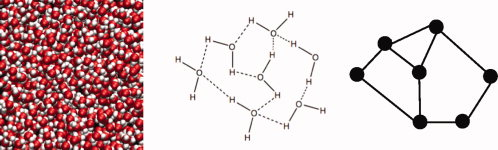
\includegraphics[width=\linewidth]{Decomposition_of_simulation_date_into_a_graph_-chem.jpg}
\caption{Decomposition of simulation data into a graph}
\label{fig:chem}
\end{figure}
\item Code with $\alpha$ set at 0.85, also can be 0.99
\item PageRank peaks influenced by number of neighbour waters
\item Lower $\alpha$ increases the influence of the neighbours
\item Each uniquely connected polyhedron has its own unique vector representation, and so able to access database for confirmation of polyhedra
\item Enhances the traditional, often non standardized methods used to extract chemical information from molecular simulation
\end{itemize}
\chapter{Roads and Urban Spaces}
\section{doi:10.1080/13658810802022822}
\begin{itemize}
\item City can be topologically represented as a connectivity graph, consisting of nodes representing individual spaces and links if the corresponding spaces are intersected
\item Can capture human movement rates in individual spaces
\item Weighted PageRank
\item PageRank scores are significantly correlated to human movement both pedestrian and vehicle in four areas of London
\begin{figure}
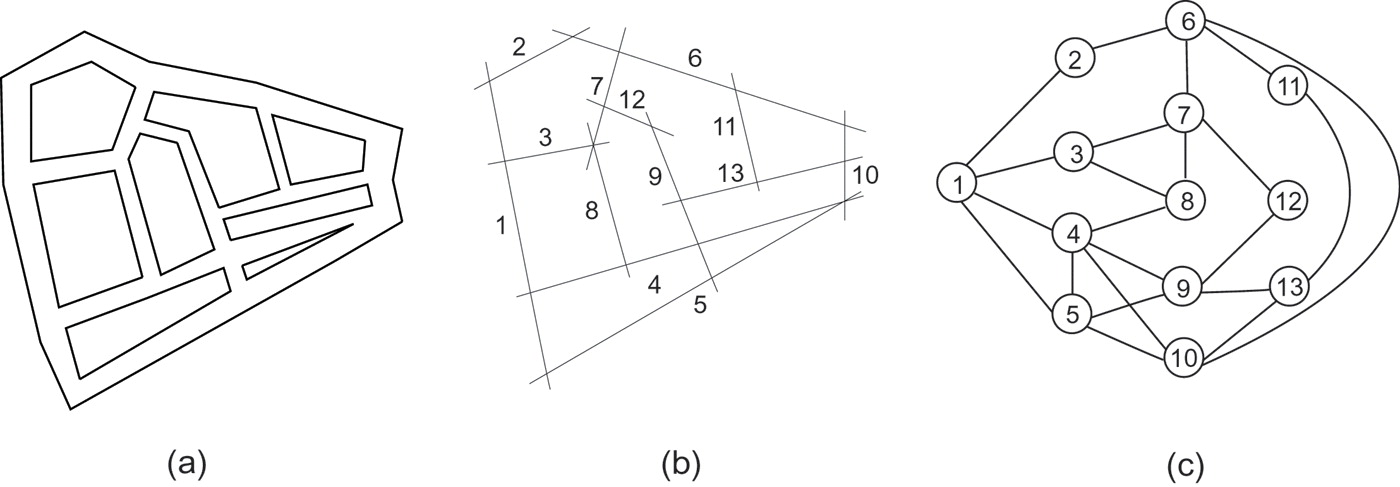
\includegraphics[width=\linewidth]{map_view.jpeg}
\caption{(a) A fictive urban system, (b) its axial map and (c) connectivity graph Source as above}
\label{fig:map}
\end{figure}
\item When applied to ranking space for an urban environment, connected and undirected graph, so no dangling nodes involved
\item Weighted PageRank score are significantly correlated to the pedestrian and vehicle flows
\item Correlation gets better as $\alpha$ increases
\item Random walker never gets stuck, and always moves to one of its successors with non-uniform probability, well-connected streets are more favourable
\item over 60\% of human movement can be predicted or explained purely from a topological point of view. In terms of statistics, the other 40\% is not predictable, and it may relate to land use, building height and road width
\item Uses a never-get-stuck-or-tired random walker
\end{itemize}
\section{1742-5468-2008-07-P07008}
\begin{itemize}
\item Weighted PageRank ($\alpha= 0.95$) is still the best metric (R square over 0.7) in terms of metric–flow correlation
\item In addition, we found that weighted PageRank with an
appropriate d factor setting tends to be one of the best metrics for correlating or predicting
traffic flow
\end{itemize}
\chapter{Recommending Systems}
\section{ItemRank: A Random-Walk Based Scoring Algorithm for Recommender Engines}
\begin{itemize}
\item Emerging technology to help consumers find interesting products
\item Makes personalized product suggestions by extracting knowledge from the previous users interactions
\item ItemRank - random-walk bases scoring algorithm used to rank products according to expected user preferences
\item ItemRank performs better than other algorithms and also less complex
\item For each user, know the ratings they've assigned
\item ItemRank - biased PageRank
\item Efficient - need around 20 iterations
\end{itemize}
\chapter{Wikipedia}
\section{Preparation of Topical Reading Lists from the Link Structure of Wikipedia}
\begin{itemize}
\item Personalized background reading lists can be generated automatically from the link structure of Wikipedia
\item Used combination localized and global PageRank
\end{itemize}
\section{Interactions of cultures and top people of Wikipedia from ranking of 24 language editions}
\begin{itemize}
\item Rank articles to find top 100 historical figures
\item Finds global historical figures
\item Find most influential cultures
\item Most of the top historical figures in Wikipedia were born in Western countries
\item Strong male skew
\item 'The reason for a somewhat unexpected PageRank leader Carl Linnaeus is related to the fact that he laid the foundations for the modern biological naming scheme so that plenty of articles about animals, insects and plants point to the Wikipedia article about him, which strongly increases the PageRank probability.'
\item Culture has high PageRank if has many inlinks from other cultures
\item  'we find for all centuries at the top positions Greek, Turkish and Arabic'
\item 'historical figures before
the 19th century, we find respectively Arabic, Turkish and Greek'
\item 'most important historical figures across Wikipedia language editions were born in Western countries after the 17th century, and are male'
\item mathematical analysis of local and global historical figures can be a useful
step towards the understanding of local and global history and interactions of world cultures
\end{itemize}
\end{document}